\Chapter{Koncepció}

A dolgozat témájának megértéséhez elsősorban érdemes betekintést nyerni a kiinduló, nem-inverz problémába is, vagyis az objektumfelismerés témakörébe. Mivel a kiinduló probléma irodalma is igen szerteágazó és igazán változatos irányokban történnek a kutatások, így csupán egy rövid áttekintő betekintést kíván nyújtani a dolgozat erre vonatkozó alfejezete.
Az inverz problémakörbe való betekintés az aktuális eredmények ismertetésével történik, amely segítséget nyújthat az inverz probléma kutatási irányainak megértésében is. A dolgozat során kialakított saját megoldásom architektúrális vázlata is bemutatásra kerül a fejezetben, amelyet az irodalomkutatás során szerzett tapasztalataim által alakítottam ki, így az aktuális eredmények ismeretében remélhetőleg könnyebben átláthatóak lesznek a kutatási folyamataim az olvasó számára.

Ezen fejezetben kerül ismertetésre továbbá a megvalósításhoz használt fejlesztői eszközök és a gépi tanulásos modellek tanításának módjai is.

\Section{Az objektumfelismerés}
Az objektumfelismerés célja a számítógépes látás esetében, hogy egy gépi tanulásos modell egy vizsgált képen meghatározza a képen található objektumokat. Egyszerűbb esetben osztályozási feladatról beszélhetünk, amely során a bemeneti képeket egy-egy diszkrét címkével látja el a modell. A modell kimeneteként rendszerint az osztályokhoz tartozó valószínűségi értékeket kaphatjuk meg. Amennyiben a képen található objektum környezetéről feltételezzük, hogy nem hordoz számunka lényeges információkat, úgy a címkék használata elegendő lehet bizonyos feladatoknál. Viszont előfordulhat olyan alkalmazási környezet is, amikor a bemeneti képeken nem csupán egyetlen objektum található és minden fellelhető objektumhoz szeretnénk címkét rendelni. Ilyen esetekben a felismert objektumokat különféle annotációkkal láthatja el a modell. Legtöbbször a megtalált objektumok pozícióiról is adhat kimenetet, az azonosított elemeket befoglaló dobozokkal \cite{redmon2016you} vagy pixel-szinten is jelölheti a modell, az utóbbi esetben szemantikus szegmentációról beszélhetünk \cite{long2015fully}.

\begin{figure}[h]
	\centering
	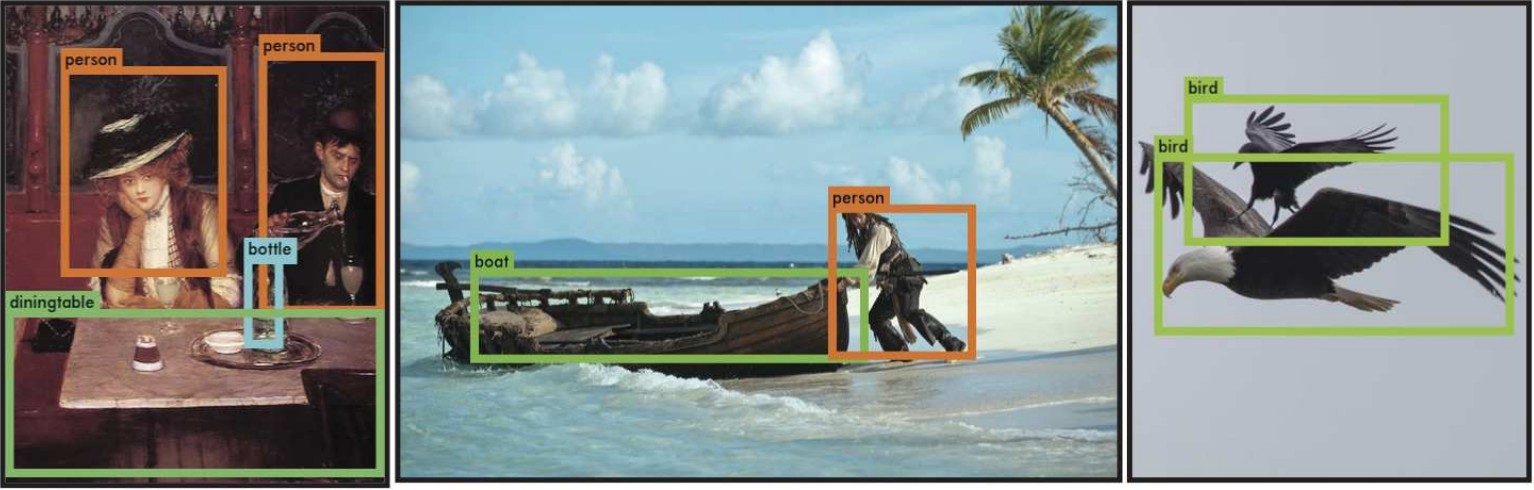
\includegraphics[width=15cm]{images/yolo.png}
	\caption{A YOLO osztályozó által megtalált befoglaló dobozok. \textit{Forrás:} \cite{redmon2016you}}
	\label{fig:yolo}
\end{figure}

A képek osztályozásához általánosságban \textit{konvolúciós} hálózatot szokás alkalmazni. A konvolúciós rétegeket tartalmazó modell ezen rétegek segítségével nyeri ki az osztályozási művelet elvégzéséhez szükséges képi-jellegzetességeket. A digitális képek $n \times m$-es mátrixokként vannak reprezentálva, a mátrix egyes pontjai pedig szürkeárnyalatos képek esetében a pixel intenzitásának értékei, színes képek esetén pedig az adott színkeverés alapján a színcsatornák értékei. A konvolúciós rétegek a kernelek és a filterek segítségével oly módon nyerik ki a bemeneti képek jellegzetességeit, hogy figyelembe veszik a pixelek szomszédságait, ezáltal a képeken található információt egy kisebb dimenziószámú leírásba transzformálja. A kisebb dimenzióban reprezentált adatokon az osztályozási feladat egyúttal könnyebben elvégezhető, másfelől a megfelelően összeállított jellegvektorok segítségével a képen található információ általánosabb formáját kapja meg az osztályozó, csökkentve annak a veszélyét, hogy a modell jellegtelen pixelekre tanulja be az egyes osztályokat.

Kiemelném az \textit{Inception modell}-t \cite{szegedy2015going}, amely a Google kutatói által kifejlesztett mély konvolúciós hálózat. Fő céljuk egy olyan modell megalkotása volt, amely az \textit{ImageNet} adathalmaz \cite{deng2009imagenet} 1000 darab osztályára megoldja az osztályozási feladatot. Az eredeti modell 2014-es megjelenése óta három további verziót is megélt (v2/v3 \cite{szegedy2016rethinking}, v4 \cite{szegedy2017inception}). A modell az inverz probléma egyes megoldásai során is szerepet kap, így a dolgozat során a későbbiekben is említésre kerül.

Az irodalomkutatás során fellelt eredmények közül a legfigyelemreméltóbb eredmény a CLIP \textit{zero-shot} osztályozó \cite{radford2021learning}, amelyet az internetről összegyűjtött képeken és a hozzájuk tartozó szöveges leírásokon tanítottak be. A CLIP modell képes rövid leírásokat adni a kép tartalmáról és az egyes mondatokat valószínűségi értékekkel látja el. Vagyis a különféle annotációk helyett természetes-nyelvi leírásokat ad kimenetként egy-egy képhez. A modell az inverz problémakör egyes megvalósításában is feltűnik majd, amelyeket a következő alfejezetben ismertetek.

%TODO: Eredmények szemléltetésére clip ábra


\Section{Az objektumfelismerés inverz problémája}

Az objektumfelismerés inverz problémája alatt azt a feladatot értjük, amely során csupán a képekre vonatkozó információk állnak rendelkezésünkre és ezen adatok alapján a gépi tanulásos modellnek a lehető legjobban kell reprezentációt találnia egy-egy kimeneti kép formájában.
Ehhez nem csupán a bemeneti, általában természetes nyelvi szöveget kell értelmeznie a modellnek, hanem a kimeneti képek előállításának módja is megoldandó feladat.
A jelenlegi eredmények alapján különféle megközelítéseket láthatunk a problémára, viszont ha csak az eredmények rendezetlen halmazára tekintünk, akkor az aktuális kutatási irányokat nehéz észrevenni. Az eredményeket többféle szempont szerint is csoportosíthatjuk az átláthatóság megkönnyítése érdekében. Mivel a megoldandó probléma alapvetően is két részre osztható: a bemeneti adatok feldolgozása és a kimeneti kép előállítása, így első körben a csoportosítást ezen két tengely mentén külön-külön is elvégezhetjük.

Ha a kimeneti képek alapján szeretnénk csoportosítani a jelenlegi eredményeket, akkor megállapíthatjuk, hogy a legtöbb szerző fotórealisztikus megjelenítésre törekedett. A képek előállítására általában \textit{generatív} modellt alkalmaztak, amely a gépi tanulásos megoldások azon halmaza, melynek feladata, hogy új adatokat állítsanak elő. Két generatív modell alkalmazása figyelhető meg a jelenlegi kutatási irányokban, azok közül is a második közkedveltebb, a talált publikációk alapján.
A képek kigenerálásához vagy \textit{Variational Autoencoder} (VAE) architektúrán alapuló modellt alkottak meg \cite{ramesh2021zero}, vagy \textit{Generative Adverserial Network} (GAN) alapú megoldásokat \cite{dong2021unsupervised, reed2016learning, xu2018attngan, zhang2017stackgan} alkalmaztak.
Egy olyan publikációt is találtam, amely figyelemreméltó módon nem generatív modellt alkalmazotta képek szintetizálására, hanem teljesen egyedi megközelítést, amelyben csupán Bézier-görbék halmazán végezték el az optimalizálást és eredményül rajzokhoz hasonló képeket kaptak. A módszert CLIPDraw-nak nevezték el \cite{frans2021clipdraw}, amelynek a nevében megtalálható, a már korábban említett CLIP osztályozó is.

A GAN és VAE részletesebb összehasonlítására egy későbbi fejezetben kerül sor. A saját módszeremhez szükséges képek előállítására szolgáló komponens alapjául, a különféle eredmények és a két módszer előnyeinek és hátrányainak figyelembe vételével úgy döntöttem, hogy egy GAN-t választom.
A GAN-hoz is igen szerteágazó kutatási irányok alakultak ki az évek során, amelyekben a közös cél természetesen az eredeti GAN kiegészítése oly módon, hogy a betanított modell a lehető legjobb eredményeket nyújtsa.

%TODO GAN hivatkozási gráf beillesztése, kis magyarázat írása az egyes irányokról és hogy mi az, amit átvettem belőlük...

\begin{figure}[h]
	\centering
	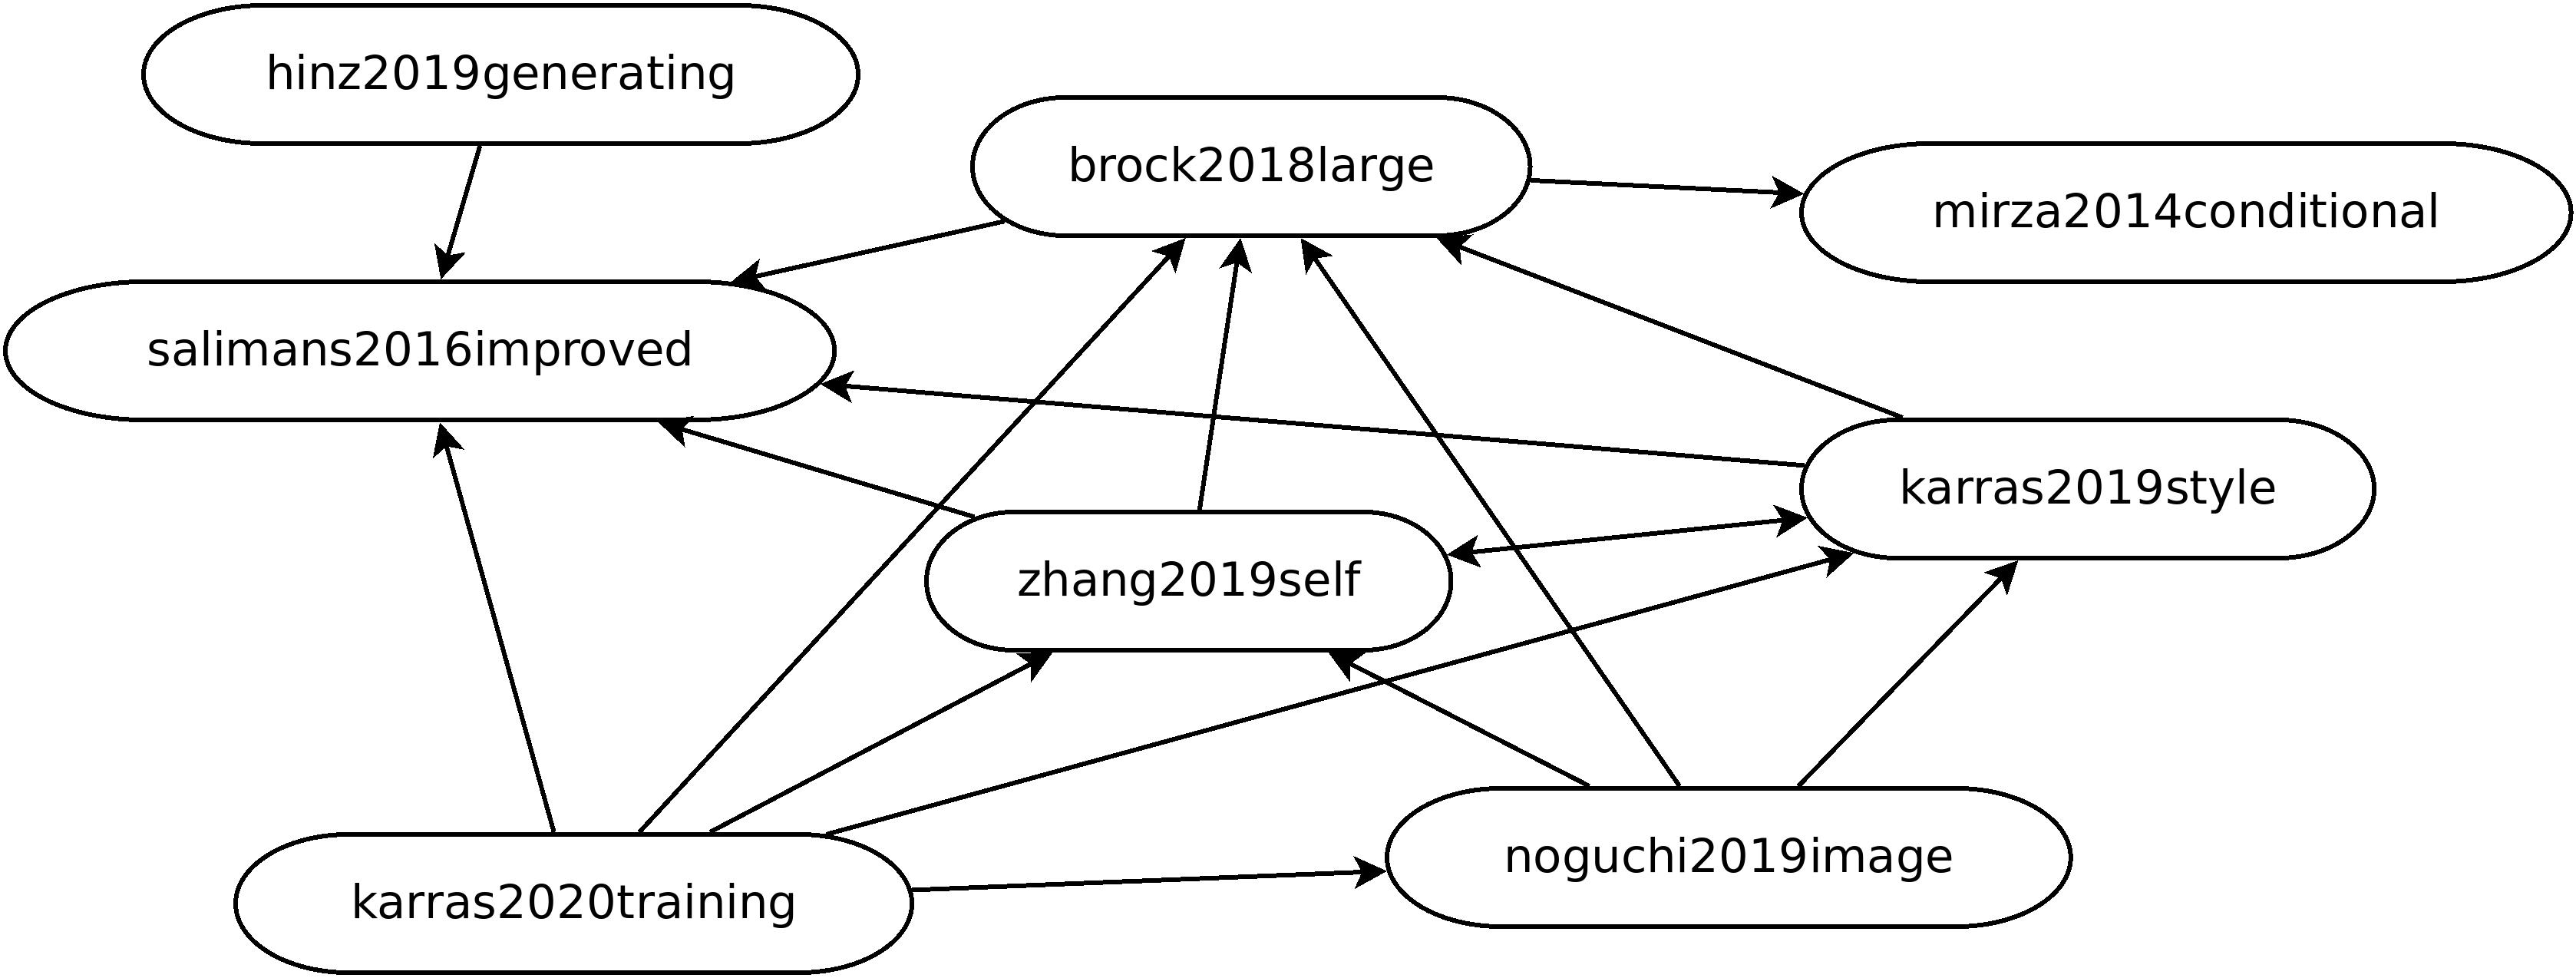
\includegraphics[width=15cm]{images/gancite.png}
	\caption{Hivatkozási gráf}
	\label{fig:gancite}
\end{figure}

% TODO: Problémakör bemutatása, különböző szerzők eredményeinek ismertetése, a képek generálásán kívül - szöveg feldolgozás és optimalizálás

\Section{Saját architektúra}

A kutatásom során szerzett ismeretek alapján a \ref{fig:architecture} ábrán szemléltetett architektúrát alkottam meg.

\begin{figure}[h]
\centering
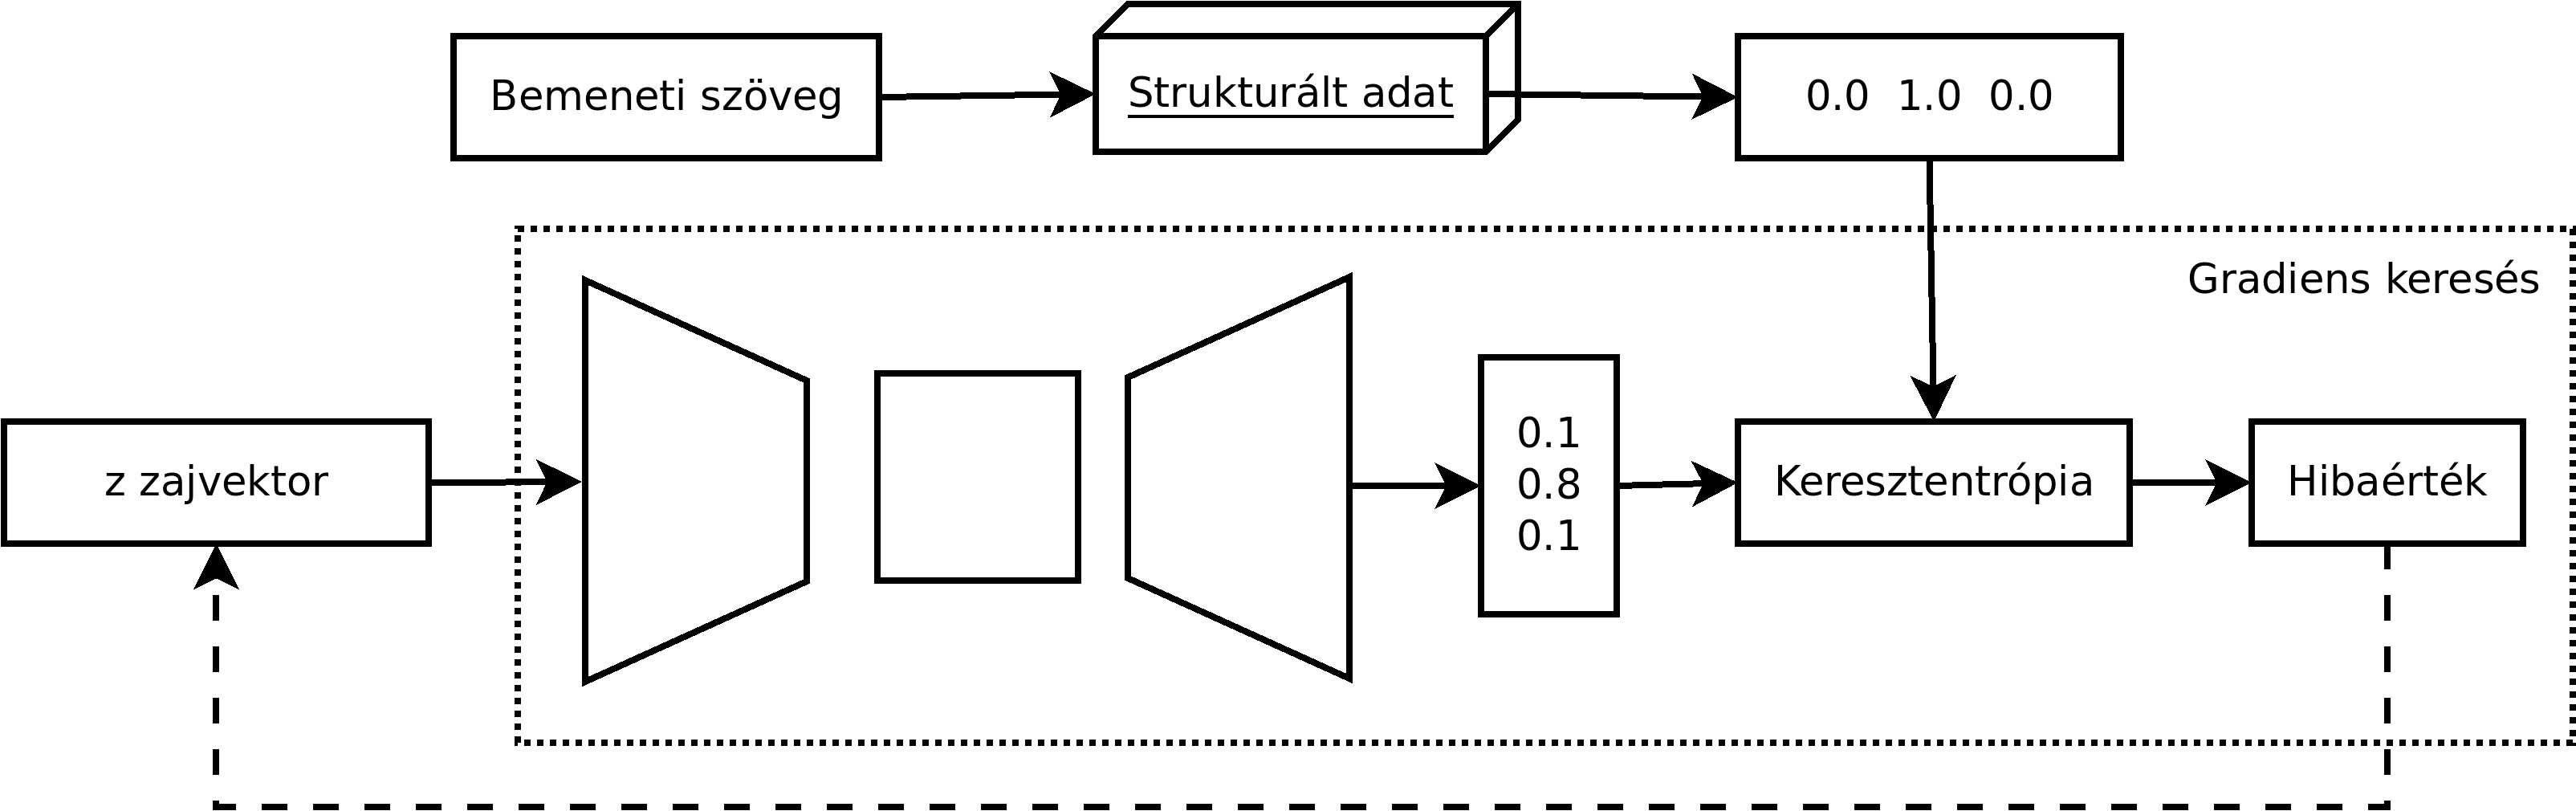
\includegraphics[width=15cm]{images/architecture.png}
\caption{Architektúra}
\label{fig:architecture}
\end{figure}

Az architektúra részei:

\begin{itemize}
	\item Bemeneti szöveg feldolgozó
	\item Strukturált adat enkódoló
	\item Optimalizáló modul
		\begin{itemize}
			\item Optimalizálandó zajvektor
			\item Képeket előállító háló (G)
			\item Osztályozó (D)
			\item Hibafüggvény számoló
		\end{itemize}
\end{itemize}

Az architektúra egy olyan zajvektort keres, amely a képeket kigeneráló háló bemeneteként a megfelelő képet előállítja.
A megoldásom egyes részei különféle megközelítési módszereken keresztül kerülnek ismertetésre a dolgozat további fejezeteiben.

%TODO: Mihez hasonlít ez? Miből mit vettem át?

\Section{Tensorflow és Keras}

A dolgozat programjának megvalósításához a TensorFlow függvénykönyvtárat választottam ki. A TensorFlow egy ingyenes, open-source gépi tanulásra használatos függvénykönyvtár, amely elsősorban mély- és gépi-tanulásos alkalmazások implementálására használatos. Számos programozási nyelvhez érhető el az API-ja, beleértve a Python, Java, C++ és JavaScript nyelveket. Viszont az API fő fejlesztési iránya a Python nyelvre összpontosul. A könyvtár a Google Brain fejlesztésében született meg 2015-ben, majd 2019-ben megjelent a 2.0-ás API verzió is, amely az API váltásból adódóan visszafelé nem teljesen kompatibilis az elsővel. Jelenleg a 2.8-as számozású stabil kiadással rendelkezik, a dokumentációja a \cite{tensorflow} forrás alatt érhető el. Az API lehetőséget ad az elosztott tanításra is. A betanított modellek széles körben alkalmazhatóak, akár web- vagy mobilalkalmazásokba is integrálhatóak. 

A Keras függvénykönyvtár egy interfészt biztosít a TensorFlowhoz. Segítségével igazán egyszerűen, modulárisan és átláthatóan állíthatunk össze neurális hálózatokat. Az általa biztosított eszközkészlet igazán változatos. A modellek összeállítására is többféle lehetőségünk van, például a \textit{Sequential API} használatával pipeline szerű modelleket építhetünk a különféle rétegek egymás után illesztésével. A \textit{Functional API} segítségével pedig igazán komplex kapcsolatokkal rendelkező architektúrák is megvalósíthatóak, a kódbonyolultság növekedése nélkül. A Keras korábban több backend-et is támogatott, viszont a legfrissebb verzióiban csak a TensorFlow-hoz alkalmazható. Látható, hogy a két könyvtár mennyire összefonódott. A dokumentációja a \cite{keras} forrás alatt érhető el.

Python-ban a \texttt{tensorflow} csomag az alábbi kódrészlettel importálható. A TensorFlow tartalmazza a Keras-t is modul formájában. Amennyiben nem importáljuk be külön a modult, úgy a \texttt{tf.keras}-al is elérhetjük, viszont az alábbi kódrészletben a Keras is importálásra kerül. A dolgozatban található kódrészleteknél az alábbi két sort nem tüntetem fel a továbbiakban, egységesen minden kódrészlethez az alábbiak szükségesek, a kivételt képző eseteknél, ahol szükséges lehet további csomagok importálása is, külön ki fogom emelni. (nem biztos, hogy lesz ilyen...)
\begin{python}
import tensorflow as tf
from tensorflow import keras
\end{python}

A dolgozathoz elkészült programokat \textit{IPython Jupyter notebook}-ok \cite{jupyter} formájában kerültek megvalósításra.

\Section{Modellek tanítása}

A mély neurális hálózatok tanítása igazán erőforrás-igényes feladat. A tanítható hiperparaméterek paraméterek nem ritkán milliós nagyságrendűek, a dataset-eknek pedig kellően nagynak kell lenniük, a feldolgozandó adatoknak pedig memóriába is bele kell férnie. Egy-egy iteráció igen sok időbe telhet egy gyengébb hardveren.

A kezdeti demóprogramok futtatása során szembesültem a első nehézséggel: A laptopom nem volt a legalkalmasabb nagyobb gépi-tanulásos modellek tanítására, hiszen igen sok időt vett igénybe a legkisebb példák futtatása is. Megoldásként egy olyan szolgáltatást kerestem az interneten, amellyel a dolgozatom programjához történő modelleket kényelmesen be tudnám tanítani.

A TensorFlow honlapján felleltem a Google Colab \cite{colab} felületet, amely ingyenes virtuális környezetet biztosít az IPython notebook-ok szerkesztéséhez és futtatásához. A felület egy előre meghatározatlan ideig GPU-t (Tesla K80) és TPU-t is biztosít kipróbálás jelleggel. Az ingyenes verzióban a napi GPU használatának limitje nincsen meghatározva, így egy idő után lekapcsolhatják és GPU nélkül megnövekszik a tanítás hossza. Továbbá a környezetet 12 óránként újraindítják, így minden adat elvezhet és csak akkor futhat a script, ha meg van nyitva a böngészőablak. Így az ingyenes verzió kisebb példák futtatására elegendő csupán és egészen korlátozott az ingyenes verzió használata. Természetesen a Tensorflow és a Keras ajánl lehetőségeket a modellek mentésére vagy a tanítás közbeni checkpoint-ok készítésére.

Például az alábbi kódrészlet futtatásával tetszőleges attribútumokkal létrehozhatunk egy checkpoint objektumot, amely segítségével mentéseket csinálhatunk a checkpoint paramétereiként megadott objektumok állapotairól. Ha esetleg a kimentett állapotokat vissza kívánjuk állítani, úgy a \texttt{checkpoint.restore()}-al a megfelelő fájlnév megadásával megtehetjük.
\begin{python}
checkpoint = tf.train.Checkpoint(
    generator_optimizer=generator_optimizer,
    discriminator_optimizer=discriminator_optimizer,
    generator=generator,
    discriminator=discriminator
)
checkpoint.save(file_prefix)

checkpoint.restore(checkpoint_path)
\end{python}

Egy másik lehetőségként lementhetjük a teljes modellt, amelyet később egyszerűen be is tölthetünk.
\begin{python}
model.save("./my_model")

new_model = keras.models.load_model("./my_model")
\end{python}
Ennek a módszernek az előnye, hogy nem szükséges a modell-t üresen deklarálni a betöltéshez, viszont a checkpoint-tal ellentétben a verziók nincsenek automatikusan menedzselve és erről nekünk kell gondoskodni. Az ilyen mentést a már betanított modellekhez javasolt megtenni, míg a checkpoint a tanítás során nyújt lehetőséget a biztonsági mentések készítésére. A saját modelleim tanítása során is felléptek olyan állapotok, amikor a modell használhatatlanná vált. Ilyen esetekben a biztonsági mentésekkel igen könnyedén vissza lehetett állítani az utolsó stabil állapotot.

Viszont számomra a Google Colab ingyenes próbaverziója nem volt teljesen megfelelő, a kiszámíthatatlanság miatt. Az előfizetés még csupán néhány kijelölt országban elérető, így Magyarországon jelenleg nem lehet a fizetős szolgáltatásra feliratkozni, így újabb felületet kellett keresnem.
Egy fórumon böngészve találtam rá a Kaggle \cite{kaggle} felületre, amely hasonló környezetet kínál, mint a Colab. Az alap. A Kaggle által biztosított virtuális környezet hardvere jobbnak bizonyult a Colab-bbal szemben. A GPU használat heti szinten kerül meghatározásra órákban, ami csak a használat során számolódik. Továbbá lehetőséget kínál a notebookok ütemezett futtatására is és az Kaggle-ön megtalálható bármelyik datasetet könnyedén betölthetjük és használhatjuk. Mindezen előnyök miatt a Kaggle-t választottam a modelljeim tanítására.

Az alábbi táblázatban található meg a laptopom és a Kaggle által biztosított környezet specifikációi:
\begin{center}
\begin{tabular}{ p{1.2cm}||p{6cm}|p{6cm}  }
	  & Dell Insprion-5558 & Kaggle környezet\\
	\hline
	\textbf{CPU} & 4x Intel(R) Core(TM) i3-5005U CPU @ 2.00GHz & 2x Intel(R) Xeon(R) CPU @ 2.00GHz\\
	\textbf{RAM} & 2x 4GB DDR3 1600 MHz & 15GB\\
	\textbf{GPU} & Intel HD Graphics 5500 (VGA) & Nvidia Tesla P100-PCIE-16GB\\
	\textbf{HDD} & 1TB & 73GB
\end{tabular}
\end{center}
A három környezet (laptop, Colab, Kaggle) teljesítményét egy általam felállított méréssel vizsgáltam.
A \texttt{RuntimeMeasure.ipynb} notebook használatos a mérés elvégzéséhez.
A teljesítménymérés alapja egy olyan GAN hálózat, amelyet meghatározott paraméterekkel hozunk létre.
A tanítás során az alábbi paraméterek változatlanok:
\begin{center}
\begin{tabular}{ c|c|c|c }
	Látens dimenziószám & mini-batch méret & filterek száma & kernelméret\\
	\hline
	100 & 32 & 128 & ($3\times 3$)
\end{tabular}
\end{center}
A felbontásnövelő rétegek száma a futó paraméter, amelyet 0-tól 3-ig vizsgálunk.
A hálózat felépítése megegyezik a DCGAN architektúrával, azzal az eltéréssel, hogy a Generátor utolsó dekonvolúciós rétege helyett egy konvolúciós réteg található, amely csupán dimenziócsökkentési feladatot végez, vagyis a feature-öket a három színcsatornába transzformálja. Hasonlóan a Diszkriminátorban is, az első konvolúciós réteg a bemeneti kép csatornáit bővíti ki, nem végez kicsinyítést.
A hálózatot 5 epoch-ig tanítjuk az adott felbontásnövelő rétegek mellett, majd az átlagos futásidő kerül lejegyzésre.
A mérés során a hálózatot a Cifar10 \cite{krizhevsky2009learning} adathalmazon tanítottam, labelek nélkül a train részhalmazán.
A mérés egyes állomásain a generátor különféle felbontásokban generálja a képeket. Így a tanítás előtt a tanítóhalmaz képeit is a generátor kimenetével megegyező méretekre kell skáláznunk.

A generátor kimenete a felbontásnövelő rétegek számával változik. Ha nem alkalmazunk ilyen réteget, akkor az ($4 \times 4$) felbontású képeket eredményez, majd rendre 1 réteg esetén ($8 \times 8$), 2 rétegnél ($16 \times 16$) és 3 rétegnél pedig ($32 \times 32$) felbontású képek jelennek meg a generátor kimenetén. A diszkriminátort is ennek megfelelően át kell alakítanunk, ott viszont a felbontáscsökkentő rétegek számát kell módosítanunk. Mivel a felvázolt GAN szimmetrikus, így a felbontásnövelő és felbontáscsökkentő rétegek száma megegyezik.

\begin{python}
...
for i in range(upsampling_layers):
    hidden = keras.layers.Conv2DTranspose(
        units_per_layer, kernel_size, 2, 'same'
    )(hidden)
    hidden = keras.layers.BatchNormalization()(hidden)
    hidden = keras.layers.ReLU()(hidden)
...
\end{python}

A generátorban és a diszkriminátorban is egy-egy for ciklussal megoldhatjuk az említett rétegek hozzáadását a hálók építésénél. A fenti példa kód szemlélteti a generátorban lévő dekonvolúciós réteg hozzáadását.
A notebookot futtatva a különböző környezeteken a \ref{fig:runtime} ábrán látható eredmények jöttek ki.

\begin{figure}[h]
\centering
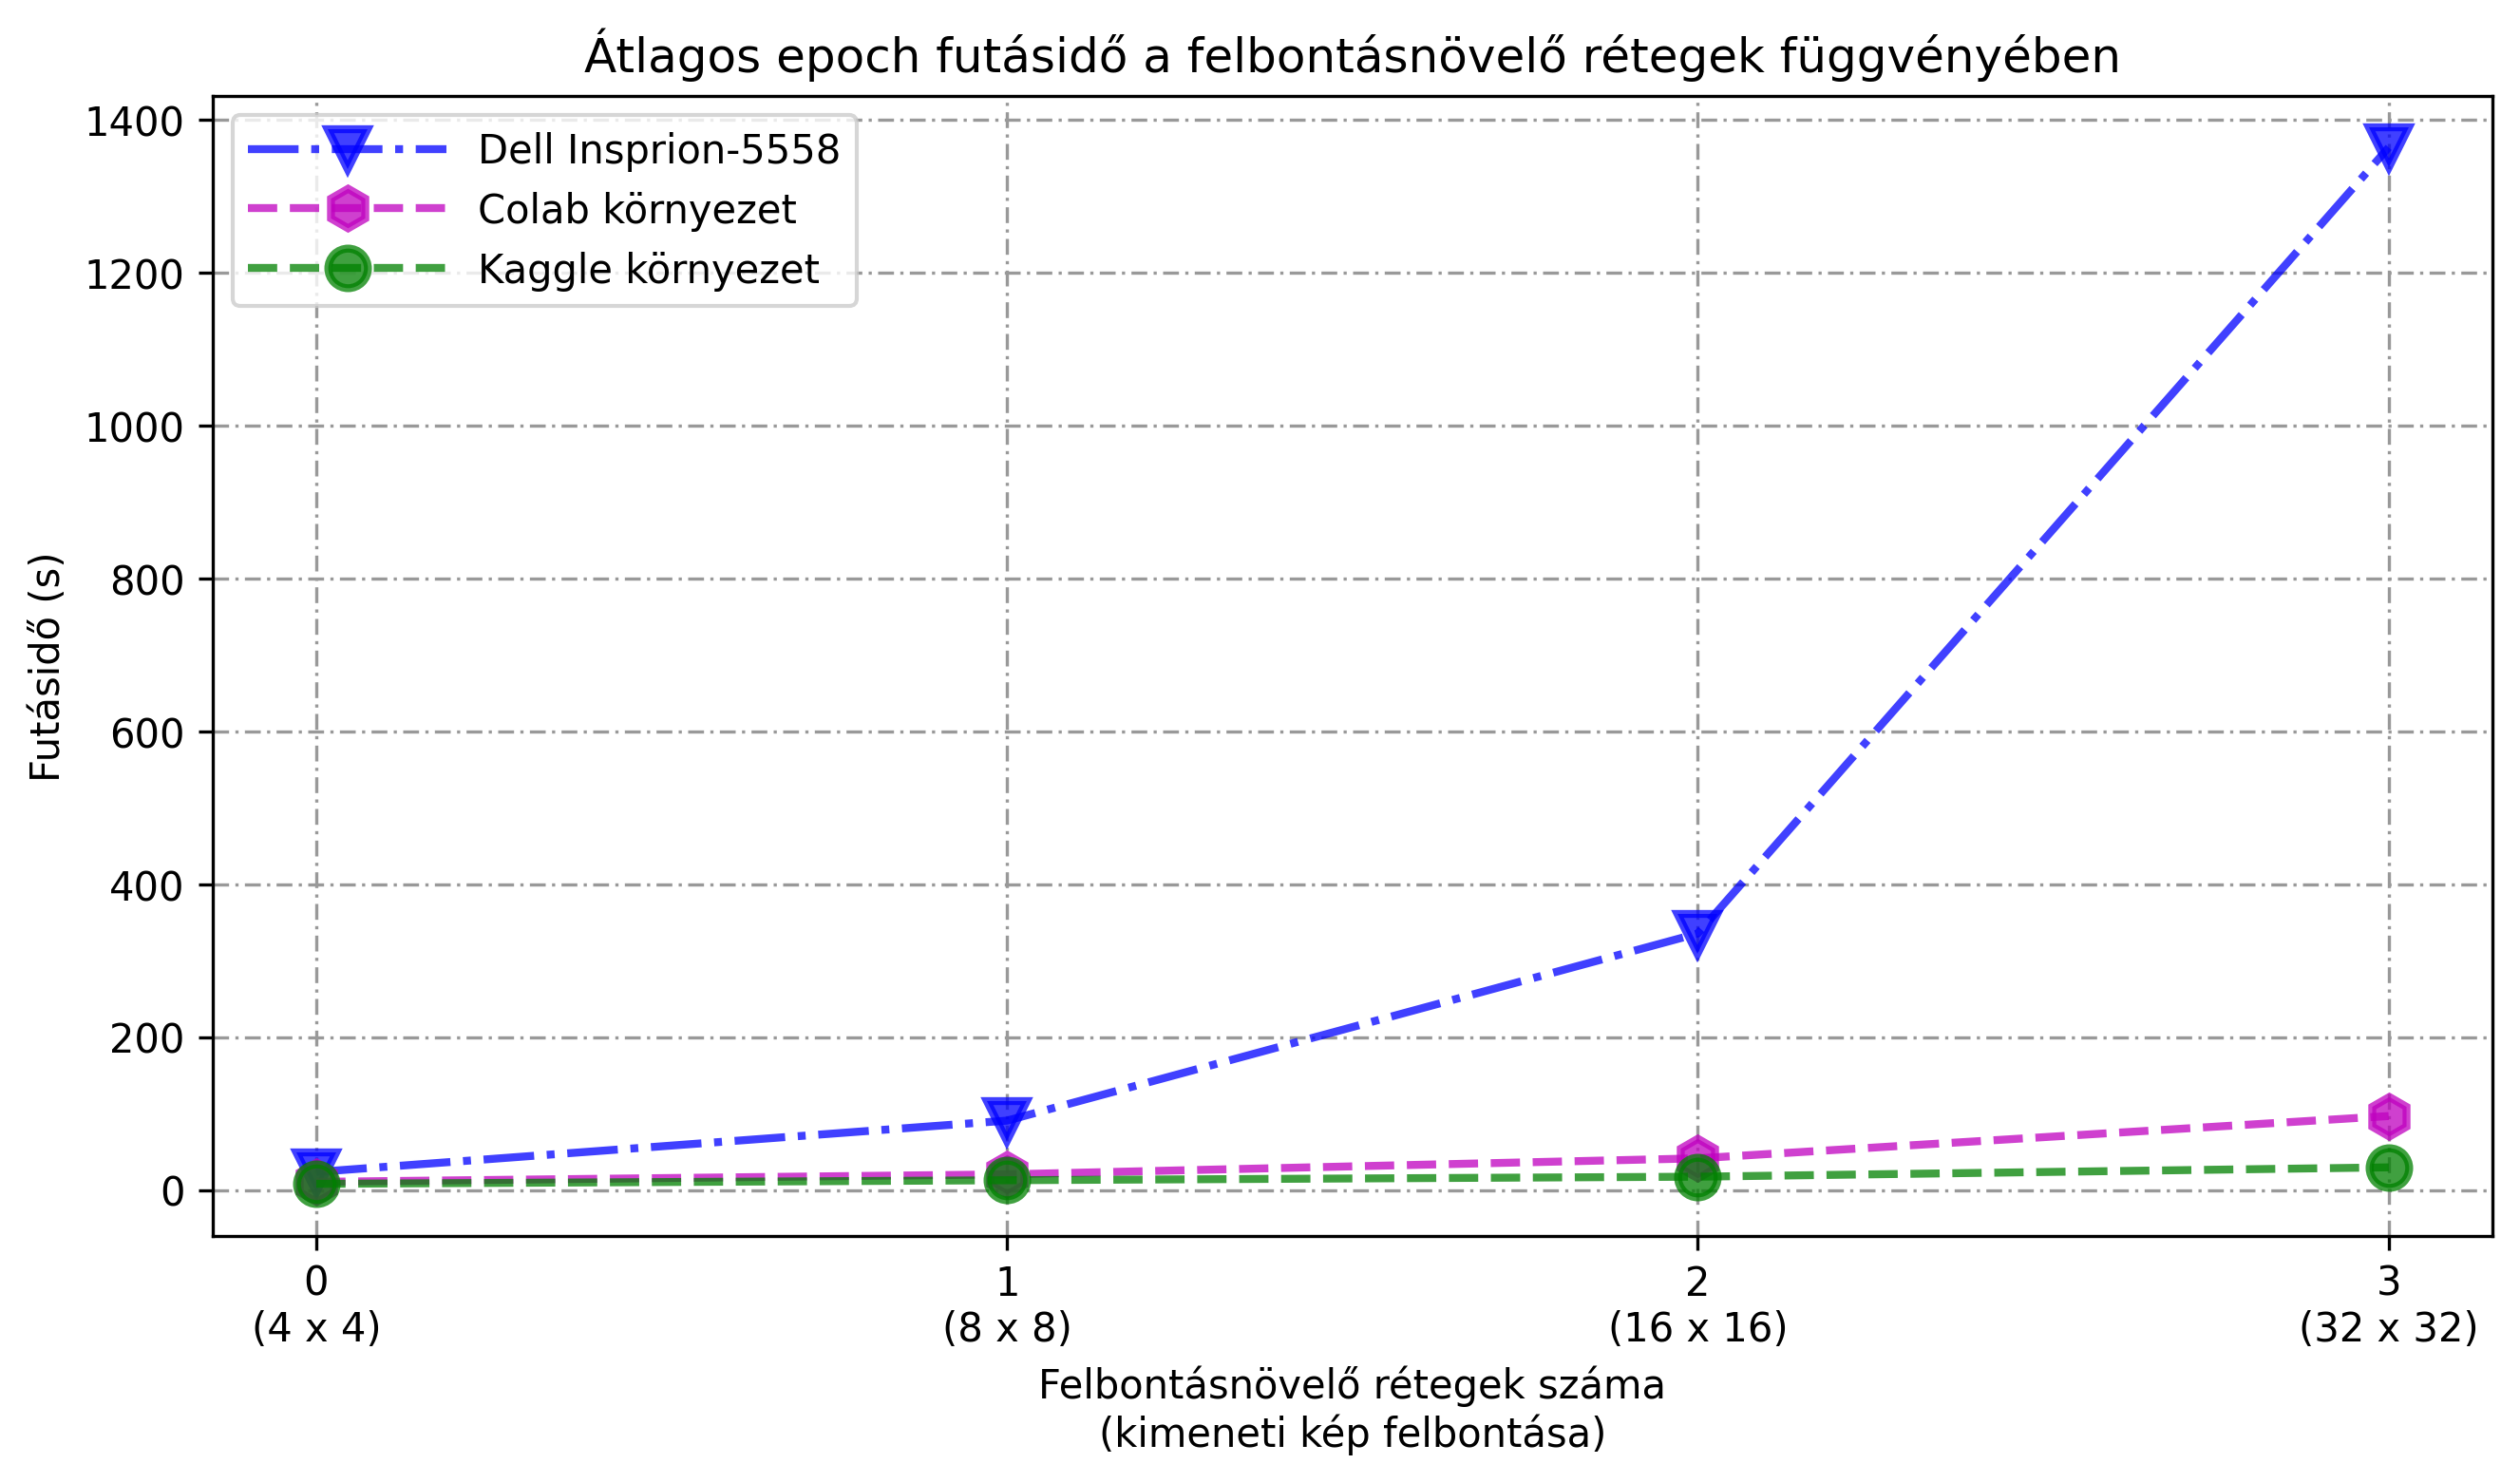
\includegraphics[width=15cm]{images/runtime.png}
\caption{Runtime ábra}
\label{fig:runtime}
\end{figure}

Mint látható, a laptopom igen alulmaradt a két virtuális környezettel szemben és érzékelteti az ábra, hogy saját munkaálláson mennyire megnehezedik a tanítás a várakozási idők meghosszabbodásával. A modellek összeállításának kezdeti fázisaiban több prototípus készült el, mire eljutottam a végleges változatig. Az egyes próbálkozások a megfelelő modell kiválasztására a laptopomon nagyon sok időt vett volna el, amely rontotta volna a kutatás hatásfokát is.

\newpage

\Section{A tanításhoz használt adathalmazok}

A tanításhoz szükségünk van egy megfelelő adathalmazra. Képek generálásához legegyszerűbb esetben elegendő lehet képek rendezetlen halmaza is és a modellre bízhatjuk, hogy ismerje fel az egyes osztályok jellegzetességeit. Megfelelő regularizációs technikákkal igazán változatos képek generálására lesz képes a betanított modell.

Ha az adathalmaz rendelkezik osztályokkal is, úgy az osztály-címkéket is felhasználhatjuk a GAN hálózatunk tanításához. Így egy plusz bemenet segítségével könnyebben tudunk majd megfelelő képeket előállítani. (Ezt a technikát class-conditioning-nak nevezik, de utána kell nézzek)

Egyes adathalmazokhoz igen részletes annotációkat is mellékelnek. A képeken megfigyelhető objektumokat határoló dobozokkal, vagy pixel szinten is jelölik. Így igen részletes információkat kínálnak a kép tartalmáról. Egy igazán hasznos annotációk lehetnek a természetes nyelvű leíró mondatok is, amelyekből általában többet is mellékelnek egy-egy képhez.

Ha kiválasztottuk a modellünkhöz megfelelő adathalmazt, akkor a probléma és a modell bonyolultságától függően elő kell készítenünk az adatokat a tanításhoz.

Az irodalomkutatás során talált egyes GAN modellek esetén megfigyelhető, hogy a fotórealisztikus eredmény érdekében a tanításhoz használt adathalmazt erősen tisztították és általában egyetlen egy doménból származnak az adatok. Tehát pédául a CelebFaces vagy az Oxford Flowers vagy a CUB esetében.

%TODO: Példák az adathalmaz elemeire, pontosítás

\begin{itemize}
	\item Animal Faces-HQ (AFHQ) \cite{choi2020stargan}\\
		Az adathalmaz állatokról tartalmaz portrékat igen jó minőségben. A színes fényképek felbontása $ 512 \times 512 $, az állatok fotói pedig pozicionálva vannak a szemük szerint. Tehát igen tisztának lehet nevezni az adathalmazt. A dataset-et bevezető publikációban azt is megemlítik, hogy kézi szelektálást is végeztek, hogy a lehető legjobb minőségű legyenek a minták. A mintákat 3 osztályban adták meg: Kutya, macska és vadállat. Az osztályokban egyenként 5000 tanítóminta található, így összesen 15 ezer képből áll az adathalmaz. A kevés osztály ellenére az osztályokon belül igen változatos képek figyelhetők meg, a fajok különböző alfajaira.
	\item Cifar-10 \cite{krizhevsky2009learning}
		A Cifar-10 adathalmaz valójában a Cifar-100 adathalmaznak egy leszűkített változata. Az utóbbi 100 osztályt magába foglaló adathalmaz, míg a Cifar-10 csupán 10 class-al rendelkezik. A tanítóhalmaza 50000 képet tartalmaz.
		Az adathalmaz képei ($32 \times 32$) felbontásúak és 3 színcsatornával rendelkeznek (RGB).
\end{itemize}
